% Options for packages loaded elsewhere
\PassOptionsToPackage{unicode}{hyperref}
\PassOptionsToPackage{hyphens}{url}
\documentclass[
]{article}
\usepackage{xcolor}
\usepackage[margin=1in]{geometry}
\usepackage{amsmath,amssymb}
\setcounter{secnumdepth}{5}
\usepackage{iftex}
\ifPDFTeX
  \usepackage[T1]{fontenc}
  \usepackage[utf8]{inputenc}
  \usepackage{textcomp} % provide euro and other symbols
\else % if luatex or xetex
  \usepackage{unicode-math} % this also loads fontspec
  \defaultfontfeatures{Scale=MatchLowercase}
  \defaultfontfeatures[\rmfamily]{Ligatures=TeX,Scale=1}
\fi
\usepackage{lmodern}
\ifPDFTeX\else
  % xetex/luatex font selection
\fi
% Use upquote if available, for straight quotes in verbatim environments
\IfFileExists{upquote.sty}{\usepackage{upquote}}{}
\IfFileExists{microtype.sty}{% use microtype if available
  \usepackage[]{microtype}
  \UseMicrotypeSet[protrusion]{basicmath} % disable protrusion for tt fonts
}{}
\makeatletter
\@ifundefined{KOMAClassName}{% if non-KOMA class
  \IfFileExists{parskip.sty}{%
    \usepackage{parskip}
  }{% else
    \setlength{\parindent}{0pt}
    \setlength{\parskip}{6pt plus 2pt minus 1pt}}
}{% if KOMA class
  \KOMAoptions{parskip=half}}
\makeatother
\usepackage{graphicx}
\makeatletter
\newsavebox\pandoc@box
\newcommand*\pandocbounded[1]{% scales image to fit in text height/width
  \sbox\pandoc@box{#1}%
  \Gscale@div\@tempa{\textheight}{\dimexpr\ht\pandoc@box+\dp\pandoc@box\relax}%
  \Gscale@div\@tempb{\linewidth}{\wd\pandoc@box}%
  \ifdim\@tempb\p@<\@tempa\p@\let\@tempa\@tempb\fi% select the smaller of both
  \ifdim\@tempa\p@<\p@\scalebox{\@tempa}{\usebox\pandoc@box}%
  \else\usebox{\pandoc@box}%
  \fi%
}
% Set default figure placement to htbp
\def\fps@figure{htbp}
\makeatother
\setlength{\emergencystretch}{3em} % prevent overfull lines
\providecommand{\tightlist}{%
  \setlength{\itemsep}{0pt}\setlength{\parskip}{0pt}}
\usepackage{amsmath}
\usepackage{amssymb}
\usepackage{amsthm}
\usepackage{booktabs}
\usepackage{longtable}
\usepackage{tikz}
\usetikzlibrary{positioning, arrows.meta, calc, shapes.misc}
\usepackage{setspace}
\usepackage{float}
\usepackage{caption}
\usepackage[round]{natbib}
\doublespacing
\newtheorem{proposition}{Proposition}
\newtheorem{corollary}{Corollary}
\newtheorem{definition}{Definition}
\usepackage{geometry}
\geometry{margin=1in}
\usepackage{booktabs}
\usepackage{longtable}
\usepackage{array}
\usepackage{multirow}
\usepackage{wrapfig}
\usepackage{float}
\usepackage{colortbl}
\usepackage{pdflscape}
\usepackage{tabu}
\usepackage{threeparttable}
\usepackage{threeparttablex}
\usepackage[normalem]{ulem}
\usepackage{makecell}
\usepackage{xcolor}
\usepackage{bookmark}
\IfFileExists{xurl.sty}{\usepackage{xurl}}{} % add URL line breaks if available
\urlstyle{same}
\hypersetup{
  pdftitle={Included Variable Bias in Dynamic Panels: A Diagnostic for Time-Varying Controls and a Benchmark for the Contemporaneous Treatment Effect},
  pdfauthor={Manoel Galdino; Davi Moreira; Carolina Dolleans},
  hidelinks,
  pdfcreator={LaTeX via pandoc}}

\title{Included Variable Bias in Dynamic Panels: A Diagnostic for
Time-Varying Controls and a Benchmark for the Contemporaneous Treatment
Effect}
\author{Manoel Galdino\footnote{Assistant Professor of Political
  Science, Universidade de São Paulo. E-mail:
  \href{mailto:mgaldino@usp.br}{\nolinkurl{mgaldino@usp.br}}} \and Davi
Moreira\footnote{Professor of Quantitative Methods, Mitch Daniels School
  of Business, Purdue University.} \and Carolina Dolleans\footnote{Graduate
  Student of Political Science, Universidade Federal de Pernambuco.}}
\date{July 2026}

\begin{document}
\maketitle
\begin{abstract}
We study included variable bias as a general diagnostic problem that
arises when researchers condition on observed covariates that may
themselves respond to treatment. Recent work on
difference-in-differences with time-varying covariates shows that in
such settings both conditioning on the realized covariate and omitting
it can be problematic, because the causally relevant object may resemble
an untreated potential covariate that is not directly observed. We
derive a closed-form included variable bias diagnostic for linear nested
models, \(\mathrm{IVB} = -\theta^{\star}\pi\), and show how directed
acyclic graphs determine whether the resulting specification shift
reflects collider bias, over-control, or deconfounding. We then develop
the paper's main applied implication: in time-series cross-sectional
settings focused on the contemporaneous treatment effect, ADL + FE with
lagged state variables provides a practical benchmark. Simulations
covering collider, dual-role, and mediator designs show that this
benchmark sharply reduces bias, blocks inherited collider paths when
outcomes are persistent, and preserves the contemporaneous total effect
when lagged rather than contemporaneous controls are used. Applications
illustrate how IVB quantifies specification shifts while the benchmark
provides a defensible starting point for applied work.
\end{abstract}

\section{Introduction}\label{introduction}

Researchers using time-series cross-sectional data constantly face a
deceptively simple specification choice: should an observed time-varying
covariate be included in the regression? Consider an
international-relations scholar studying the effect of UN peacekeeping
on democratization. Conditioning on conflict intensity is tempting
because more severe conflicts are more likely to receive peacekeeping
missions and are less likely to democratize. But peacekeeping can itself
reduce violence. If so, conditioning on contemporaneous conflict
intensity means conditioning on a variable that may already have
responded to treatment. Omitting conflict may leave confounding;
including realized conflict may introduce a different problem. The same
logic appears whenever researchers want to control for GDP, aid,
inflation, turnout, repression, or any other variable that evolves
within the same period as treatment and outcome.

Recent work on difference-in-differences with time-varying covariates
makes this problem stark. When a covariate can itself respond to
treatment, both conditioning on the realized covariate and omitting it
can be problematic, because the causally relevant object may be
something like the untreated potential covariate \(Z_t(0)\) rather than
the realized \(Z_t\)
\citep{caetano_callaway2024, caetano_etal2022, lin_zhang2022}. Related
work on panels and causal dynamics likewise shows that time-varying
covariates can create demanding identification problems
\citep{blackwell2018make, imai_kim2021}. We take that broader literature
as the starting point rather than the target of critique.

Our contribution is different and narrower, but also more operational.
We introduce included variable bias (IVB) as a general diagnostic
problem that arises when researchers condition on observed covariates
that may themselves respond to treatment. In linear nested models, the
resulting specification shift admits a simple closed-form decomposition:
\[
\widehat{\beta}^{\star} - \widehat{\beta} = - \widehat{\theta}^{\star}\widehat{\pi},
\] where \(\widehat{\theta}^{\star}\) is the coefficient on the
candidate control in the long regression and \(\widehat{\pi}\) is the
coefficient on treatment in an auxiliary regression for that control.
Directed acyclic graphs (DAGs) tell the researcher what kind of variable
\(Z\) is; IVB tells the researcher how much including it moves the
treatment coefficient. This is the paper's general contribution. The
current manuscript develops it for the linear models most common in TSCS
work, where the diagnostic is exact and directly estimable.

The paper's main applied payoff is narrower. For TSCS settings focused
on the contemporaneous treatment effect (CET), the IVB logic and the
associated timing argument imply a practical benchmark: start from ADL +
FE with lagged state variables, use lagged covariates when substantively
justified, and treat contemporaneous time-varying controls as suspect
until the timing is explicit. This is not the claim that ADL solves
every panel-data problem. It is the claim that, for the CET, ADL + FE
provides a defensible baseline when controlling correctly for
time-varying covariates would otherwise require stronger and often
untestable assumptions.

This architecture helps distinguish the paper from two nearby
contributions. It is not only a warning that time-varying controls are
hard, because IVB gives that difficulty a named and estimable
diagnostic. And it is not only a recommendation to use dynamic
specifications, because the benchmark is presented as the main applied
implication of a more general included-variable-bias framework. The
broader research program behind IVB may well travel beyond the current
setting, but this paper develops its full payoff in the linear TSCS
case.

We proceed in four steps. Section\textasciitilde{}\ref{sec:control}
defines the control-variable problem when observed covariates may
themselves respond to treatment.
Section\textasciitilde{}\ref{sec:timing} uses DAG logic to show why the
same substantive variable can be harmful at \(t\) and useful at \(t-1\).
Section\textasciitilde{}\ref{sec:ivb} presents IVB as the paper's
general diagnostic contribution and derives the closed-form
decomposition used in linear TSCS models.
Section\textasciitilde{}\ref{sec:benchmark} then develops the main
applied implication of that framework: a benchmark for the CET based on
ADL + FE with lagged state variables.
Section\textasciitilde{}\ref{sec:applications} shows how IVB and the
benchmark interact in published TSCS studies.
Section\textasciitilde{}\ref{sec:conclusion} closes with the paper's
claim, its limits, and the agenda it opens.

\section{\texorpdfstring{The Time-Varying Control Problem for the
Contemporaneous Treatment Effect
\label{sec:control}}{The Time-Varying Control Problem for the Contemporaneous Treatment Effect }}\label{the-time-varying-control-problem-for-the-contemporaneous-treatment-effect}

Applied researchers working with time-series cross-sectional (TSCS) data
rarely face a binary choice between
\texttt{control\textquotesingle{}\textquotesingle{}\ and}do not
control.'\,' The more realistic problem is whether an observed
time-varying covariate should enter the specification when the estimand
is the contemporaneous treatment effect (CET), that is, the effect of
\(D_t\) on \(Y_t\). The same variable can help, hurt, or redefine the
estimand depending on timing. A contemporaneous covariate \(Z_t\) may be
a confounder, a collider, or a mediator. Its lag, \(Z_{t-1}\), may
instead behave as a predetermined state variable relative to the CET.

Standard heuristics are too coarse for this problem.
\texttt{Control\ checking\textquotesingle{}\textquotesingle{}\ recommends\ adding\ predictors\ of\ the\ outcome\ to\ gain\ precision;}confounding
checking'\,' recommends adding joint causes of treatment and outcome
\citep{cinelli2021crash}. Both heuristics ignore the possibility that a
candidate control is post-treatment in the period of interest. That
omission is costly in TSCS designs because treatment, outcome, and
covariates evolve jointly over time, often with persistence in all three
processes \citep{blackwell2018make, imai_kim2021}.

Recent DID work sharpens the problem further: if \(Z_t\) may itself
respond to treatment, neither conditioning on realized \(Z_t\) nor
omitting it necessarily identifies the target estimand, because the
relevant object may be the untreated potential covariate \(Z_t(0)\)
rather than the observed \(Z_t\)
\citep{caetano_callaway2024, caetano_etal2022}. We do not solve that
identification problem in general. Instead, we ask a more operational
question. When applied researchers condition on an observed time-varying
covariate that may respond to treatment, how much does that choice move
the treatment coefficient, and what is the safest default specification
in the TSCS case?

Our answer has two parts. The general contribution is IVB: a named
diagnostic problem and an exact decomposition for linear nested models.
The more specific contribution is the paper's payoff in TSCS settings
with the CET: a dynamic benchmark based on ADL + FE with lagged state
variables. In other words, the paper is not only about a safer
specification rule and not only about a formula. It is about how the
formula makes the safer rule operational.

The scope qualification matters. A lagged control is pre-treatment only
relative to the effect of \(D_t\) on \(Y_t\). That does not make it
universally innocuous for cumulative, delayed, or long-run effects. The
paper's positive recommendation is therefore explicitly local to the
CET. Difference-in-differences and related panel designs remain part of
the motivation for why time-varying controls are hard, but the paper's
formal and applied results are developed in the linear TSCS setting.

\section{\texorpdfstring{DAGs, Timing, and Why \(Z_t\) Is Not
\(Z_{t-1}\)
\label{sec:timing}}{DAGs, Timing, and Why Z\_t Is Not Z\_\{t-1\} }}\label{dags-timing-and-why-z_t-is-not-z_t-1}

The causal role of a time-varying covariate is inseparable from its time
index. For the CET, \(Z_t\) is contemporaneous with both treatment and
outcome. That is exactly where post-treatment bad controls live. By
contrast, \(Z_{t-1}\) precedes \(D_t\) and \(Y_t\), so it can operate as
a lagged state variable even when \(Z_t\) is a collider or mediator.

\subsection{Preliminaries}\label{preliminaries}

\begin{figure}[H]
\centering
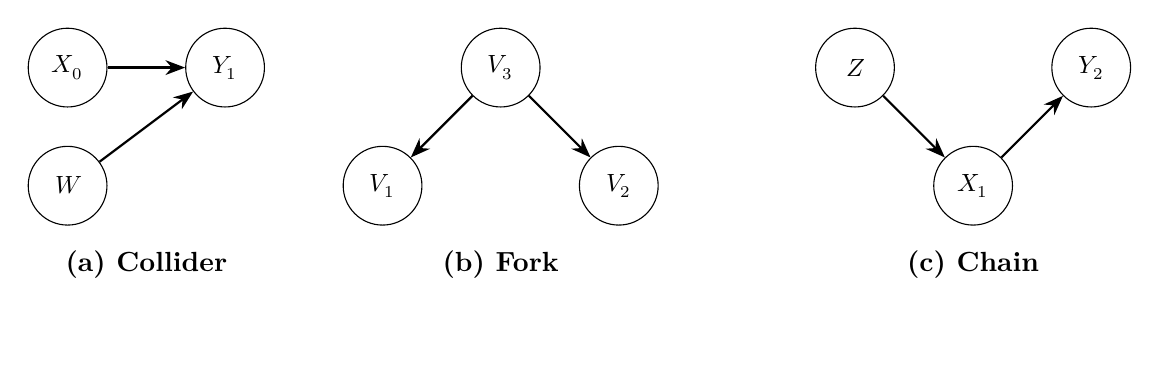
\begin{tikzpicture}[
    node distance=1.8cm,
    every node/.style={draw, circle, minimum size=1cm, font=\small},
    arr/.style={-{Stealth[length=2.5mm]}, thick}
]

\node (X0) at (0,4) {$X_0$};
\node (Y1) at (2,4) {$Y_1$};
\node (W) at (0,2.5) {$W$};
\draw[arr] (X0) -- (Y1);
\draw[arr] (W) -- (Y1);
\node[draw=none, font=\normalsize\bfseries] at (1, 1.5) {(a) Collider};

\node (V3) at (5.5,4) {$V_3$};
\node (V1) at (4,2.5) {$V_1$};
\node (V2) at (7,2.5) {$V_2$};
\draw[arr] (V3) -- (V1);
\draw[arr] (V3) -- (V2);
\node[draw=none, font=\normalsize\bfseries] at (5.5, 1.5) {(b) Fork};

\node (Z) at (10,4) {$Z$};
\node (X1) at (11.5,2.5) {$X_1$};
\node (Y2) at (13,4) {$Y_2$};
\draw[arr] (Z) -- (X1);
\draw[arr] (X1) -- (Y2);
\node[draw=none, font=\normalsize\bfseries] at (11.5, 1.5) {(c) Chain};

\end{tikzpicture}
\caption{The three elementary DAG structures. For the CET, the practical question is whether a candidate control behaves like a fork at $t-1$ or like a collider or mediator at $t$.}
\label{fig:three_structures_pa}
\end{figure}

Forks, chains, and colliders remain the fundamental building blocks
\citep{pearl2009causality, elwert2014endogenous}. What changes in TSCS
work is that the same substantive variable can move across these roles
as we shift its time index. A lagged income measure may be a fork that
blocks omitted variable bias; contemporaneous income may instead be a
mediator or collider if both treatment and outcome affect it within
period \(t\).

\subsection{Timing Logic for Candidate
Controls}\label{timing-logic-for-candidate-controls}

Table\textasciitilde{}\ref{tab:timing_logic} summarizes the main timing
logic. The key point is that the paper's benchmark is anchored to the
CET rather than to a generic slogan such as ``lag everything.'\,'

\begin{table}[!h]
\centering
\caption{\label{tab:timing-logic-table}Timing logic for observed controls when the estimand is the contemporaneous treatment effect. The same substantive variable can move from bad control at $t$ to useful state variable at $t-1$. \label{tab:timing_logic}}
\centering
\resizebox{\ifdim\width>\linewidth\linewidth\else\width\fi}{!}{
\begin{tabular}[t]{llll}
\toprule
Candidate.control & Likely.role.for.the.CET & Main.risk.or.benefit & Default.action\\
\midrule
$Z_t$ & Collider & Opens a backdoor path & Do not condition unless the DAG rules out post-treatment status\\
$Z_t$ & Mediator & Blocks part of the total effect & Do not condition if the target is the total contemporaneous effect\\
$Z_{t-1}$ & Predetermined state & Captures state dependence & Candidate benchmark control\\
$Z_{t-1}$ & Lagged confounder & Removes OVB without blocking the contemporaneous path & Candidate benchmark control\\
\bottomrule
\end{tabular}}
\end{table}

Three cases are especially relevant for the remainder of the paper.
First, a contemporaneous collider \(Z_t\) opens a backdoor path and
creates IVB. Second, a contemporaneous mediator \(Z_t\) creates
over-control if the target is the total contemporaneous effect. Third, a
dual-role variable can be both a lagged confounder and a contemporaneous
collider. In that case, the empirical question is not whether the
variable should ever appear in the specification, but whether it should
enter as \(Z_t\) or as \(Z_{t-1}\).

\section{\texorpdfstring{The Included Variable Bias Diagnostic
\label{sec:ivb}}{The Included Variable Bias Diagnostic }}\label{the-included-variable-bias-diagnostic}

The paper's general contribution is to define included variable bias as
a distinct diagnostic problem. Once researchers accept that an observed
control may itself respond to treatment, they need a language for the
resulting specification shift. DAGs classify the control. IVB quantifies
what that classification means for the treatment coefficient in a given
linear specification.

Consider the short model \begin{equation}
Y = \beta D + W \delta + u
\label{eq:short_pa}
\end{equation} and the long model \begin{equation}
Y = \beta^{\star} D + \theta^{\star} Z + W \delta^{\star} + u^{\star},
\label{eq:long_pa}
\end{equation} where \(W\) collects admissible controls. By the
Frisch--Waugh--Lovell theorem, \begin{equation}
\widehat{\beta}^{\star} - \widehat{\beta} = - \widehat{\theta}^{\star} \widehat{\pi},
\label{eq:ivb_main_pa}
\end{equation} where \(\widehat{\pi}\) is the coefficient on \(D\) in
the auxiliary regression of \(Z\) on \(D\) and \(W\). In cross-sections,
\(W\) may contain baseline covariates. In TSCS settings, \(W\) can
include fixed effects, lagged dependent variables, lagged treatment, and
other lagged state variables. The formula is therefore an exact
linear-model identity, not a separate estimator. That exactness is what
makes IVB useful as more than a metaphor: the diagnostic can be read
directly off nested linear regressions already familiar to applied
researchers.

Two interpretive points matter. First, the formula is diagnostic rather
than self-justifying. If \(Z\) is a confounder, the same arithmetic
difference reflects deconfounding rather than harm. If \(Z\) is a
mediator, the difference reflects movement from the total to the direct
effect \citep{acharya_etal2016}. Only the DAG tells the researcher which
interpretation applies. Second, the formula remains useful precisely
because it converts a vague modeling dispute into two estimable
components: how strongly \(Z\) predicts the outcome in the long model,
and how strongly \(D\) predicts \(Z\) once admissible controls have been
partialled out.

This is also where the paper's originality lies. Work on dynamic
identification, sequential ignorability, and DID with time-varying
covariates shows why observed controls may be problematic
\citep{blackwell2018make, imai_kim2021, caetano_callaway2024}. IVB
contributes a different object: a named and estimable decomposition of
the specification shift itself. The current paper develops that object
in the linear TSCS domain, where it yields both a diagnostic and, in the
next section, a practical benchmark. Whether analogous IVB diagnostics
can be built for synthetic-control-style estimators, synthetic DID, or
factor models is an important agenda, but not a result claimed here.

For the CET in TSCS settings, the practically relevant auxiliary
regression is dynamic. If the benchmark specification is
\begin{equation}
Y_{it} = \beta D_{it} + \rho Y_{i,t-1} + \kappa D_{i,t-1} + X_{i,t-1}'\lambda + \alpha_i + \tau_t + \varepsilon_{it},
\label{eq:benchmark_pa}
\end{equation} then the corresponding IVB decomposition asks how much
the treatment coefficient shifts when a candidate control is moved from
the lagged-state set \(X_{i,t-1}\) into the contemporaneous set. This is
the operational meaning of ``diagnosing bad controls'\,' in the
remainder of the paper.

The formula also clarifies a point that is easy to miss in practice:
lagging the treatment is not a mechanical cure. If \(D_t\) is
autocorrelated, a collider that is contemporaneous with \(D_t\) can
remain associated with \(D_{t-1}\). What matters is not whether the
treatment index moved backward by one period, but whether the
specification blocks the transmission of the bad-control path for the
estimand of interest.

\section{\texorpdfstring{Benchmarking Dynamic Specifications for the CET
\label{sec:benchmark}}{Benchmarking Dynamic Specifications for the CET }}\label{benchmarking-dynamic-specifications-for-the-cet}

This section develops the paper's main applied implication of the IVB
framework. For the CET, the default applied comparison should be between
dynamic specifications that differ in whether they condition on
contemporaneous \(Z_t\), not between a dynamic model and a static TWFE
short regression treated as a causal gold standard. The benchmark is
therefore not a substitute for IVB. It is the most important operational
payoff of IVB in the TSCS setting studied here.

\subsection{Collider and Dual-Role Controls in
TSCS}\label{collider-and-dual-role-controls-in-tscs}

We begin with the dual-role setting in which \(Z_{t-1}\) is a confounder
for \((D_t, Y_t)\), but \(Z_t\) is contemporaneously affected by both
treatment and outcome. This is the empirically common case in which a
variable such as GDP is useful as a lagged state variable but dangerous
as a contemporaneous control.

\begin{figure}[H]

{\centering \includegraphics[width=0.85\linewidth]{ivb_paper_pa_files/figure-latex/dual-role-bias-figure-1} 

}

\caption{Dual-role simulation: ADL + FE with lagged state variables dominates static alternatives. In the main design, ADL + FE + $Z_{t-1}$ keeps bias near zero across the full range of collider persistence, while TWFE remains biased even when it includes $Z_{t-1}$.}\label{fig:dual-role-bias-figure}
\end{figure}

The message is sharp. In the main dual-role design, the bias of ADL + FE
+ \(Z_{t-1}\) stays between 0.008 and 0.010, while the bias of TWFE +
\(Z_{t-1}\) remains between 0.237 and 0.271. The static short model
performs worst, reaching 0.716 in the most persistent scenarios. The
substantive implication is that the right comparison is not ``control
versus no control'\,' in the abstract. It is whether the researcher
treats \(Z\) as a lagged state variable inside a dynamic model or as a
contemporaneous regressor in a model that omits the dynamic state.

The crucial mechanism is outcome persistence. The inherited collider
path created by conditioning on \(Z_{t-1}\) only becomes bias in the CET
equation when the spurious association can propagate from \(Y_{t-1}\) to
\(Y_t\). Table\textasciitilde{}\ref{tab:firewall_pa} shows that once
outcome persistence is shut down, the TWFE bias essentially disappears.

\begin{table}[!h]
\centering
\caption{\label{tab:firewall-table}Outcome persistence is what makes the inherited collider path bite. When $\rho_Y = 0$, the bias from conditioning on $Z_{t-1}$ is essentially zero even without $Y_{t-1}$. When $\rho_Y > 0$, adding $Y_{t-1}$ restores the benchmark. \label{tab:firewall_pa}}
\centering
\resizebox{\ifdim\width>\linewidth\linewidth\else\width\fi}{!}{
\begin{tabular}[t]{rrr}
\toprule
Outcome persistence ($\rho_Y$) & TWFE + $Z_{t-1}$ & ADL + FE + $Z_{t-1}$\\
\midrule
0.0 & 0.001 & 0.008\\
0.5 & 0.251 & 0.009\\
0.8 & 0.261 & 0.004\\
\bottomrule
\end{tabular}}
\end{table}

This finding disciplines the paper's recommendation. The lagged outcome
is not a magical fix. It matters because it blocks the transmission of
spurious dependence when the outcome process is persistent. In the
dual-role design, the practical benchmark is therefore ADL + FE with
lagged state variables, including \(Y_{t-1}\) and substantively
justified lags of candidate controls.

\subsection{Over-Control with Contemporaneous
Mediators}\label{over-control-with-contemporaneous-mediators}

The second recurring problem is not collider bias but over-control. When
\(Z_t\) lies on the path from \(D_t\) to \(Y_t\), conditioning on
\(Z_t\) shifts the estimate toward the direct effect. For the CET, the
right benchmark is again dynamic: compare an ADL specification that
leaves the contemporaneous mediator out of the regression with one that
conditions on \(Z_t\), and ask whether a lagged version \(Z_{t-1}\) can
enter the benchmark without blocking the contemporaneous path.

\begin{table}[!h]
\centering
\caption{\label{tab:overcontrol-table}Over-control simulations for the CET. In both the pure-mediator and mediator-plus-confounder designs, conditioning on contemporaneous $Z_t$ pulls the estimate toward the direct effect, whereas conditioning on $Z_{t-1}$ preserves the contemporaneous total effect. \label{tab:overcontrol_pa}}
\centering
\resizebox{\ifdim\width>\linewidth\linewidth\else\width\fi}{!}{
\begin{tabular}[t]{lrrrrr}
\toprule
Scenario & Target total & Target direct & ADL total & ADL bad ($Z_t$) & ADL safe ($Z_{t-1}$)\\
\midrule
Pure mediator, $\rho_Z = 0.3$ & 1.20 & 1 & 1.201 & 0.998 & 1.199\\
Pure mediator, $\rho_Z = 0.7$ & 1.20 & 1 & 1.199 & 0.992 & 1.197\\
Mediator + confounder, $\rho_Z = 0.5$ & 1.03 & 1 & 1.091 & 1.023 & 1.031\\
Mediator + confounder, $\rho_Z = 0.7$ & 1.03 & 1 & 1.111 & 1.016 & 1.028\\
\bottomrule
\end{tabular}}
\end{table}

The clean mediator design is the simplest illustration. ADL total
recovers the true contemporaneous total effect of about 1.20, ADL bad
(\(Z_t\)) lands near the direct effect of 1.00, and ADL safe
(\(Z_{t-1}\)) remains essentially equal to the total effect. The general
design strengthens the same conclusion. When \(Z_{t-1}\) is also a
confounder, including it improves the estimate by removing lagged
omitted variable bias without blocking the contemporaneous path
\(D_t \rightarrow Z_t \rightarrow Y_t\).

This is why TWFE short is not the right benchmark for the mediator case.
A static specification without the relevant dynamics mixes over-control
with omitted dynamics, making the comparison harder rather than easier
to interpret. The operational contrast should instead be ADL total
versus ADL bad versus ADL safe.

\subsection{Practical Benchmark}\label{practical-benchmark}

The evidence above yields a simple rule for applied TSCS work centered
on the CET:

\begin{enumerate}
\def\labelenumi{\arabic{enumi}.}
\tightlist
\item
  Start from an ADL + FE specification with lagged state variables,
  including \(Y_{t-1}\) and any substantively justified lagged controls.
\item
  Treat any contemporaneous time-varying covariate \(Z_t\) as a
  potential bad control until the DAG rules out collider and mediator
  status.
\item
  Use the IVB decomposition to quantify the shift in the treatment
  coefficient when a candidate control is included.
\item
  Interpret that shift through the DAG: collider, mediator, confounder,
  or dual-role variable.
\item
  Revisit the benchmark if the estimand is not the CET. A control that
  is pre-treatment for the CET need not be innocuous for long-run or
  cumulative effects.
\end{enumerate}

Additional simulations sharpen the scope of this recommendation. When
the outcome equation contains nonlinear effects of \(Z_{t-1}\) or
level-dependent trends of the kind emphasized in the recent DID
literature, the bias of ADL(all) never exceeds 0.4 percent of \(\beta\)
across stable scenarios. These are therefore not practical boundary
conditions for the benchmark in our TSCS setting. By contrast, ADL(all)
does not resolve contemporaneous unobserved confounding. In simulations
where an unobserved variable affects both \(D_t\) and \(Y_t\) in the
same period, the bias of ADL(all) ranges from 8 to 53 percent of
\(\beta\), while an oracle specification that observes the confounder
keeps bias below 0.3 percent. The benchmark therefore addresses
included-variable bias and related timing problems, not classical
endogeneity from unobserved contemporaneous confounding.

This benchmark is intentionally narrower than a universal recommendation
for all panel estimators. It is a defensible default for the specific
but common problem the paper studies: deciding what to do with observed
time-varying controls when the goal is the contemporaneous treatment
effect.

\section{\texorpdfstring{Applications
\label{sec:applications}}{Applications }}\label{applications}

The applications serve two purposes. First, they show that IVB yields
interpretable empirical diagnostics rather than only theoretical
algebra. Second, they show how the TSCS benchmark disciplines the
interpretation of those diagnostics. Across 14 collider candidates in
six studies, the median \(|\mathrm{IVB}/\mathrm{SE}|\) is 0.13, and only
1 case exceeds one standard error. That pattern is consistent with the
simulation evidence: many applied settings contain candidate bad
controls, but dynamic benchmarking and careful timing often keep the
practically relevant distortion modest.

\subsection{\texorpdfstring{Application 1: Democracy and Ethnic
Inequality
\label{sec:app_leipziger_pa}}{Application 1: Democracy and Ethnic Inequality }}\label{application-1-democracy-and-ethnic-inequality}

\citet{leipziger2024} estimates the effect of democratization on ethnic
inequality with a two-way fixed-effects design that includes lagged GDP
per capita. In the reframed paper, the practical question is whether GDP
should be treated as a lagged confounder, a lagged bad control, or a
dual-role variable.

GDP per capita is a plausible dual-role variable in this setting.
Democratization can raise income over time
\citep{acemoglu_etal2019, papaioannou_siourounis2008}, while ethnic
inequality can depress income through weaker public-goods provision and
conflict channels \citep{grundler_link2024}. The IVB decomposition
therefore does not mechanically tell us to drop GDP. It tells us what
the treatment estimate pays for including it.

\begin{table}[!h]
\centering
\caption{\label{tab:leipziger-ivb-table}IVB decomposition for Leipziger (2024), public-services inequality measure.}
\centering
\resizebox{\ifdim\width>\linewidth\linewidth\else\width\fi}{!}{
\begin{tabular}[t]{ll}
\toprule
Component & Estimate\\
\midrule
$\hat\beta_{\text{short}}$ & -0.0407\\
$\hat\beta_{\text{long}}$ & -0.0352\\
$\hat\theta^{\star}$ & -0.0497\\
$\hat\pi$ & 0.1123\\
IVB $= -\hat\theta^{\star}\hat\pi$ & 0.0056\\
\addlinespace
$|\mathrm{IVB}/\mathrm{SE}|$ & 0.48\\
$|\mathrm{IVB}|/|\hat\beta_{\text{long}}|$ & 15.9\%\\
\bottomrule
\end{tabular}}
\end{table}

The estimated IVB is 0.0056, or about 0.48 standard errors. The
treatment effect is attenuated by roughly 16 percent, but the shift
remains well within ordinary sampling uncertainty. This is a useful
example of the paper's practical stance: a candidate dual-role control
can matter substantively without overturning the empirical conclusion.

\subsection{\texorpdfstring{Application 2: Postal Infrastructure and
Economic Growth
\label{sec:app_rogowski_pa}}{Application 2: Postal Infrastructure and Economic Growth }}\label{application-2-postal-infrastructure-and-economic-growth}

\citet{rogowski_etal2022} provide the complementary case. Their
country-panel growth regression includes lagged GDP per capita, which is
both a plausible collider and a textbook growth confounder. Here the IVB
formula reveals a large arithmetic shift but cannot decide, by itself,
whether dropping GDP improves identification.

\begin{table}[!h]
\centering
\caption{\label{tab:rogowski-ivb-table}IVB decomposition for Rogowski et al. (2022).}
\centering
\resizebox{\ifdim\width>\linewidth\linewidth\else\width\fi}{!}{
\begin{tabular}[t]{lrrrrrrr}
\toprule
Control as $z$ & $\hat\beta_{\text{short}}$ & $\hat\beta_{\text{long}}$ & $\hat\theta^{\star}$ & $\hat\pi$ & IVB & $|\mathrm{IVB}/\mathrm{SE}|$ & IVB/$\hat\beta$ (\%)\\
\midrule
Log GDP p.c. & 0.0083 & 0.0198 & -4.0130 & 0.0029 & 0.0115 & 2.11 & 58.0\\
Log population & 0.0206 & 0.0198 & -1.9465 & -0.0004 & -0.0008 & 0.15 & -4.0\\
Urbanization & 0.0192 & 0.0198 & -3.1421 & 0.0002 & 0.0006 & 0.11 & 3.0\\
Polity2 & 0.0191 & 0.0198 & 0.0341 & -0.0221 & 0.0008 & 0.14 & 3.8\\
\bottomrule
\end{tabular}}
\end{table}

For lagged GDP per capita, \(|\mathrm{IVB}/\mathrm{SE}| = 2.11\), the
largest value among the published applications. But this is precisely
the case in which the formula must not be overread. GDP is a plausible
collider because postal infrastructure is part of the paper's
development mechanism and growth cumulates into future income levels. It
is also a plausible confounder because of conditional convergence. The
lesson is not ``drop GDP.'\,' The lesson is that a large specification
shift demands explicit causal reasoning about timing and role. This is
exactly the use case for IVB in a paper whose applied payoff is a
benchmark rather than an automatic decision rule.

\section{\texorpdfstring{Conclusion
\label{sec:conclusion}}{Conclusion }}\label{conclusion}

This paper introduces included variable bias as a general diagnostic
problem that arises when researchers condition on observed covariates
that may themselves respond to treatment. In the linear nested models
used throughout TSCS work, IVB admits a simple closed-form
decomposition. That decomposition does not decide whether a control is
admissible; DAGs and timing do that work. But it does quantify the size
and direction of the resulting specification shift in a way that
existing discussions of time-varying controls typically do not.

The paper's main applied payoff is narrower and more concrete. For TSCS
settings focused on the contemporaneous treatment effect, the IVB
framework implies a practical benchmark: ADL + FE with lagged state
variables. That benchmark is not a universal solution for all panel
estimators, nor is it a claim that lagged controls are always innocuous.
It is a defensible starting point for the specific setting studied here.
The simulations show why it works in the cases most likely to worry
applied researchers: dual-role controls, inherited collider paths, and
contemporaneous mediators.

This combination of a general diagnostic and a specific benchmark is the
paper's contribution. Without IVB, the paper would risk collapsing into
a familiar recommendation to use dynamic specifications. Without the
benchmark, IVB would risk remaining an algebraic curiosity. Put
together, they provide both a language for the problem and an
operational default for a common applied setting.

The limits are equally important. The benchmark is local to the CET. A
lagged covariate that is pre-treatment for \(D_t \rightarrow Y_t\) need
not be harmless for distributed, cumulative, or long-run effects.
Additional simulations further show that the benchmark remains robust to
nonlinear effects of lagged controls and level-dependent trends, but not
to persistent unobserved contemporaneous confounding. And although the
IVB idea may extend beyond the current domain, this paper does not claim
results for synthetic-control-style estimators, synthetic DID, or factor
models. Extending IVB to those settings is an important agenda for
future work. The present paper establishes the idea and its main payoff
in the linear TSCS case.

\singlespacing
\bibliographystyle{apsr}
\bibliography{references}

\end{document}
